\chapter{Simulation-Based Inference}\index{simulation-based inference}

You survey 20 classmates about how much they sleep, and the average is 6.8 hours. How far
off from the true average for your whole school might that be? A friend runs an
experiment and finds that students who studied in silence scored 2 points higher on a quiz
than students who studied with music. Is that a real effect, or could it be luck?

Statisticians have formulas for questions like these, and the next chapters teach them. But
the ideas behind the formulas are simpler than the formulas themselves, and with a computer
you can use the ideas directly. This chapter shows two techniques that answer both
questions with nothing but resampling and shuffling: the \newterm{bootstrap} and the
\newterm{permutation test}. They were invented only about 50 years ago, once computers became
fast enough, and today they are everyday tools in science and data analysis.

\section{The Bootstrap}\index{bootstrap}
In the Sampling Distributions and the Central Limit Theorem chapter, we learned how much a
sample mean varies by drawing thousands of samples from a population. In real life, you
cannot do that: you have one sample, and the population is unknown.

The bootstrap's trick is to let the sample stand in for the population. If the sample was
chosen at random, it is our best picture of what the population looks like. So we draw new
samples \emph{from the sample}, of the same size, \textbf{with replacement}. Each
\newterm{bootstrap sample} uses the same values, but some appear twice or more and some not
at all, just as a fresh random sample from the population would contain different people.
Computing the statistic for thousands of bootstrap samples shows how much it bounces around.
The name comes from the phrase ``pulling yourself up by your own bootstraps'': the sample
estimates its own uncertainty.

\textbf{Example}: Twenty randomly chosen students report how many hours they slept. Estimate the
average for the whole school, with a range of plausible values.

\begin{minted}{python}
import numpy as np

rng = np.random.default_rng(4)

# Hours of sleep reported by 20 randomly chosen students
sleep = np.array([6.5, 7.0, 5.5, 8.0, 6.0, 7.5, 6.5, 9.0, 5.0, 7.0,
                  6.0, 8.5, 7.0, 6.5, 4.5, 7.5, 6.0, 7.0, 8.0, 6.5])
n = len(sleep)
print(f"sample mean: {sleep.mean():.3f}")

# 10,000 bootstrap samples: n values drawn WITH replacement from the sample
resamples = rng.choice(sleep, size=(10_000, n), replace=True)
boot_means = resamples.mean(axis=1)

low, high = np.percentile(boot_means, [2.5, 97.5])
print(f"bootstrap SE: {boot_means.std():.3f}")
print(f"s / sqrt(n):  {sleep.std(ddof=1) / np.sqrt(n):.3f}")
print(f"95% bootstrap interval: ({low:.2f}, {high:.2f})")
\end{minted}
\begin{verbatim}
sample mean: 6.775
bootstrap SE: 0.250
s / sqrt(n):  0.253
95% bootstrap interval: (6.28, 7.25)
\end{verbatim}

\begin{figure}[H]
\centering
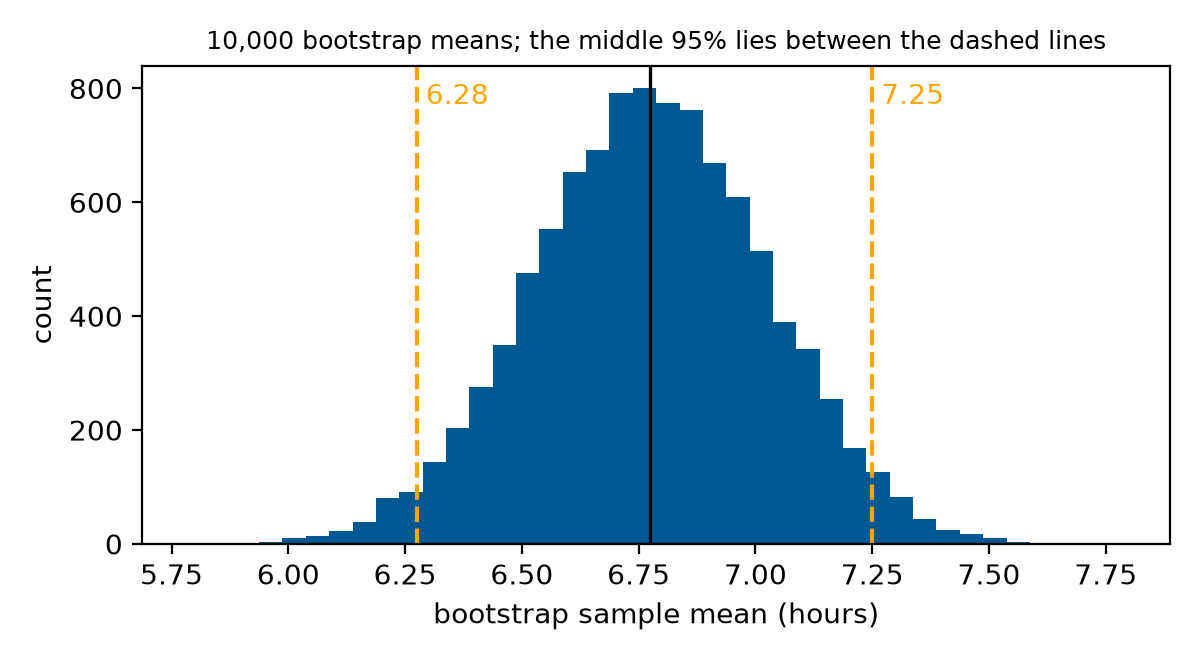
\includegraphics[width=0.75\textwidth]{bootstrap.png}
\caption{The bootstrap distribution of the sample mean. The black line is the original
sample mean, and the dashed lines cut off the lowest and highest 2.5\%.}
\label{fig:bootstrap}
\end{figure}

Three things to notice:
\begin{itemize}
\item The bootstrap means pile up in a bell shape around the sample mean, just as the CLT
predicts.
\item Their standard deviation, the \newterm{bootstrap standard error}, is 0.250 hours. The CLT
chapter's formula $\frac{\sigma}{\sqrt{n}}$, using the sample's standard deviation $s$ in place of the
unknown $\sigma$, gives 0.253. The simulation rediscovered the formula.
\item The middle 95\% of the bootstrap means runs from 6.28 to 7.25 hours. This is a
\newterm{95\% bootstrap percentile interval}: a range of plausible values for the school's true
average sleep. We are fairly confident the true average is somewhere in it. The next chapter
calls this kind of range a \emph{confidence interval} and gives formulas for it.
\end{itemize}

\subsection{Beyond the Mean}
The real power of the bootstrap is that the same code works for any statistic, even ones with no
simple formula. Change one line to bootstrap the \emph{median}, the 90th percentile, or the
correlation between two variables, and you get an interval for that too. Statisticians with only
formulas would be stuck.

\subsection{What the Bootstrap Cannot Do}
The bootstrap can only reuse the information already in the sample. If the sample was not random
(say, you asked only your friends), resampling it thousands of times reproduces the same bias
thousands of times. And with a very small sample, a handful of values cannot represent the
population's shape well, so the bootstrap interval can be too narrow. Random sampling still comes
first.

\begin{Exercise}[title={Bootstrap Samples by Hand}, label=si_hand]
A tiny sample has the values 3, 5, and 8.
\begin{enumerate}
\item Write down three different possible bootstrap samples.
\item Can a bootstrap sample be $8, 8, 8$? Can it be $3, 5, 9$? Explain.
\item What is the largest possible bootstrap sample mean?
\end{enumerate}
\end{Exercise}
\begin{Answer}[ref=si_hand]
\begin{enumerate}
\item For example, $3, 5, 8$; $5, 5, 3$; and $8, 3, 8$. Each has three values drawn with replacement
from $\{3, 5, 8\}$.
\item Yes, $8, 8, 8$ is possible, because values are drawn with replacement. No, $3, 5, 9$ is
impossible, because 9 is not in the original sample.
\item 8, from the bootstrap sample $8, 8, 8$.
\end{enumerate}
\end{Answer}

\begin{Exercise}[title={Bootstrapping a Median}, label=si_median]
Change \filename{bootstrap.py} to compute a 95\% bootstrap interval for the median hours of sleep.
(Hint: \mintinline{python}{np.median(resamples, axis=1)}.)
\end{Exercise}
\begin{Answer}[ref=si_median]
\begin{minted}{python}
import numpy as np

rng = np.random.default_rng(6)
sleep = np.array([6.5, 7.0, 5.5, 8.0, 6.0, 7.5, 6.5, 9.0, 5.0, 7.0,
                  6.0, 8.5, 7.0, 6.5, 4.5, 7.5, 6.0, 7.0, 8.0, 6.5])
resamples = rng.choice(sleep, size=(10_000, len(sleep)), replace=True)
boot_medians = np.median(resamples, axis=1)
print(np.median(sleep), np.percentile(boot_medians, [2.5, 97.5]))
\end{minted}
The sample median is 6.75 hours, and the 95\% bootstrap interval is from 6.25 to 7.25 hours.
(The bootstrap medians can only take a few values here, because the data are all multiples of 0.5.)
\end{Answer}

\section{The Permutation Test}\index{permutation test}
Now the experiment. Twenty-four students were randomly assigned to study for a quiz either in
silence or with music, 12 in each group.
\begin{center}
\begin{tabular}{l|l}
Silence & 15, 17, 14, 16, 18, 13, 17, 15, 16, 19, 14, 16 \\
\hline
Music & 13, 15, 12, 16, 14, 11, 15, 13, 17, 14, 12, 15
\end{tabular}
\end{center}
The silence group's mean is 15.83 and the music group's is 13.92, a difference of 1.92 points.

Here is the skeptic's argument. ``Music makes no difference. Each student would have gotten the
same score in either group. The groups differ only because of which students the random assignment
happened to put where.'' That claim is the \newterm{null hypothesis}.

If the skeptic is right, the labels ``silence'' and ``music'' are meaningless. So we can test the
claim directly: pool all 24 scores, shuffle them, deal them into two new groups of 12, and compute
the difference in means. That is one \newterm{permutation}. Repeat 10,000 times, and you see what
differences random assignment alone produces when music truly does nothing.

\begin{minted}{python}
import numpy as np

rng = np.random.default_rng(5)

# Quiz scores (out of 20) in a randomized experiment
silence = np.array([15, 17, 14, 16, 18, 13, 17, 15, 16, 19, 14, 16])
music   = np.array([13, 15, 12, 16, 14, 11, 15, 13, 17, 14, 12, 15])
observed = silence.mean() - music.mean()
print(f"observed difference: {observed:.3f}")

# If music makes no difference, the labels are meaningless: shuffle them.
scores = np.concatenate([silence, music])
diffs = np.empty(10_000)
for i in range(10_000):
    shuffled = rng.permutation(scores)
    diffs[i] = shuffled[:12].mean() - shuffled[12:].mean()

p_value = np.mean(diffs >= observed)
print(f"p-value: {p_value:.4f}")
\end{minted}
\begin{verbatim}
observed difference: 1.917
p-value: 0.0083
\end{verbatim}

\begin{figure}[H]
\centering
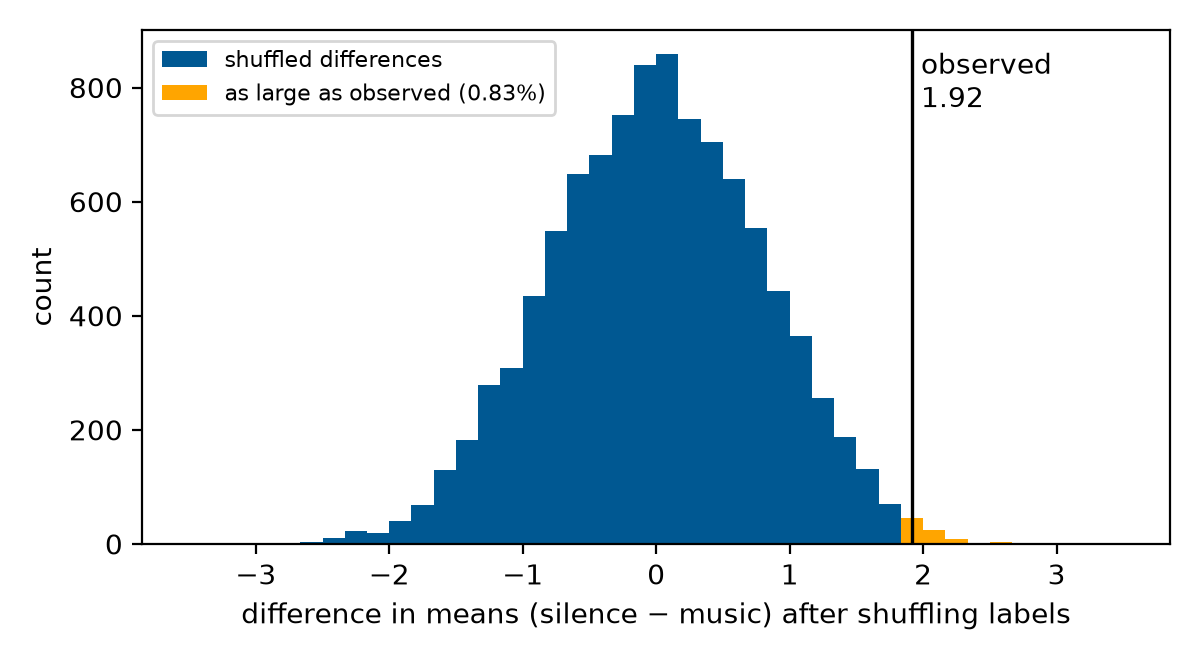
\includegraphics[width=0.75\textwidth]{permutation.png}
\caption{Differences in means after shuffling the labels 10,000 times. Only 0.83\% of the shuffles
produced a difference as large as the real one.}
\label{fig:permutation}
\end{figure}

The shuffled differences cluster around 0, as they should if labels do not matter. A difference of
1.92 or more came up in only 83 of the 10,000 shuffles. That fraction, 0.0083, is the
\newterm{p-value}: the probability, if music makes no difference, of seeing a difference at least as
large as the one observed. It is so small that the skeptic's story is hard to believe. We have
convincing evidence that, for students like these, studying in silence leads to higher quiz scores.
Because the groups were formed by random assignment, the difference was caused by the music, not by
some other difference between the groups.

The Statistical Inferences for Means chapter later in this volume teaches a formula-based version of this test,
the two-sample $t$-test. For these data, it gives a p-value of about 0.007, close to our
simulation's 0.008.

\subsection{Why Shuffling Works}
Shuffling is not a trick; it repeats the experiment's own randomness. The random assignment is the
only reason the two groups could differ if music had no effect. By re-doing the assignment thousands
of times, we build the distribution of differences that the null hypothesis predicts, with no
formulas and no assumptions about bell curves. That is why permutation tests are trusted even for
small samples and skewed data.

\begin{Exercise}[title={A New Warm-Up Routine}, label=si_prop]
A coach randomly assigns 40 runners to a new warm-up routine or the old one, 20 each. In the new
group, 10 runners improved their times; in the old group, 4 did. Write a permutation test to estimate
the p-value for the claim that the new routine helps. What do you conclude?
\end{Exercise}
\begin{Answer}[ref=si_prop]
\begin{minted}{python}
import numpy as np

rng = np.random.default_rng(7)
# 1 = improved, 0 = did not; first 20 got the new routine, last 20 the old one
outcomes = np.array([1] * 10 + [0] * 10 + [1] * 4 + [0] * 16)
observed = 10 - 4          # 6 more students improved with the new routine

diffs = np.empty(10_000)
for i in range(10_000):
    shuffled = rng.permutation(outcomes)
    diffs[i] = shuffled[:20].sum() - shuffled[20:].sum()
print(np.mean(diffs >= observed))
\end{minted}
It prints a p-value of about 0.047. If the routine made no difference, a gap of 6 or more improvers
would happen only about 5\% of the time, so this is some evidence that the new routine helps, though
not overwhelming. (This is right at the usual 0.05 cutoff, which the next chapters explain.)
\end{Answer}

\begin{Exercise}[title={What the p-Value Means}, label=si_meaning]
A student says, ``The p-value of 0.0083 means there is a 0.83\% chance that music has no effect.''
Explain what is wrong with that statement, and give a correct interpretation.
\end{Exercise}
\begin{Answer}[ref=si_meaning]
The p-value is computed \emph{assuming} music has no effect, so it cannot be the probability of that
assumption. Correct: if music had no effect on quiz scores, only about 0.83\% of random assignments
would produce a difference in means of 1.92 points or more.
\end{Answer}

\begin{Exercise}[title={Bootstrap or Permutation?}, label=si_which]
For each question, say whether a bootstrap or a permutation test fits better.
\begin{enumerate}
\item From a random sample of 50 phone users, estimate the median daily screen time with a range of
plausible values.
\item In a randomized experiment, did plants given a new fertilizer grow taller than plants given
plain water?
\end{enumerate}
\end{Exercise}
\begin{Answer}[ref=si_which]
\begin{enumerate}
\item Bootstrap: you want an interval for one statistic (the median) from one sample.
\item Permutation test: you want to know whether a difference between two randomly assigned groups is
larger than chance alone would produce.
\end{enumerate}
\end{Answer}
